\documentclass{article}
\usepackage{graphicx}
\usepackage{polski}
\usepackage{listings}
\usepackage{titling}
\usepackage{subcaption}
\usepackage{placeins} % Required for \FloatBarrier

\renewcommand{\lstlistingname}{Kod}

% Definicja polecenia do dodawania podtytułu

\newcommand{\subtitle}[1]{
  \posttitle{
    \par\end{center}
    \begin{center}\large#1\end{center}
    \vskip0.5em}
}

\title{Raport}
\author{Szymon Twardosz, Dominik Jeżów}
\subtitle{rekurencyjna kompresja macierzy z wykorzystaniem częściowego SVD}

\date{\today}

\begin{document}

\maketitle

\section{\'Srodowisko}
Do wykonania \'cwiczenia wykorzystali\'smy język
python 3.11 wraz z nast\k{e}puj\k{e}cymi bibliotekami
numpy, matplotlib, sklearn oraz time

\section{Temat zadania}

Zadanie polegało na zaimplementowaniu i przetestowaniu rekurencyjnej metody korzystającej z częściowego SVD. Dodatkowo, należało stworzyć narzędzie umożliwiające wizualizację skompresowanej macierzy.

Proces testowania obejmował generowanie serii 5-elementowych dużych macierzy z różnym stopniem zagęszczenia, kolejno: 1\%, 2\%, 5\%, 10\%, 20\%. Następnie, po wygenerowaniu każdej macierzy, mierzone były czasy kompresji SVD dla dwóch różnych dopuszczalnych rzędów macierzy.

Dodatkowo, należało zaimplementować funkcję dekompresującą i ocenić, jak bardzo różni się oryginalna macierz od zdekompresowanej.

\section{Pseudokod}
\begin{lstlisting}[language=Python]
  CreateTree(tmin, tmax, smin, smax, r, epsilon):
      U, D, V = truncatedSVD(A(tmin:tmax ; smin:smax))
      if D[r+1, r+1] < epsilon:
          v = CompressMatrix(tmin, tmax, smin, smax, U, D, V, r)
      else:
          v = new node
          v.append(CreateTree(tmin, tnewmax, smin, snewmax))
          v.append(CreateTree(tmin, tnewmax, snewmax+1, smax))
          v.append(CreateTree(tnewmax+1, tmax, smin, snewmax))
          v.append(CreateTree(tnewmax+1, tmax, snewmax+1, smax))
      return v            
\end{lstlisting}


Jak widać w powyższym pseudokodzie, pierwszym krokiem jest próba skompresowania pewnego fragmentu macierzy za pomocą techniki SVD. Następnie, w zależności od jakości uzyskanej kompresji, podejmujemy decyzję, czy zachować tę kompresję, czy też dokonać kompresji na cztery mniejsze fragmenty.
\section{Ważniejsze fragmenty kodu}
\begin{lstlisting}[language=Python]
  def create_tree(matrix, r, epsilon):
  U, s, V = randomized_svd(matrix, n_components=r)
  
  node = None
  if s[-1] < epsilon:
      node = compress_matrix(matrix, U, s, V, r)
  
  else:
      Y, X = matrix.shape
      
      if Y == X == 1: # cannot segment matrix
          node = CompressNode(rank=1, size=(1, 1))
          node.val = matrix
          return node
      
      node = CompressNode(rank=r, children=[], size=(Y, X))
      
      # 4 childrens
      
      node.append_child(create_tree(matrix[0: Y // 2, 0: X // 2], r, epsilon))
      node.append_child(create_tree(matrix[0: Y // 2, X // 2: X], r, epsilon))
      node.append_child(create_tree(matrix[Y // 2: Y, 0: X // 2], r, epsilon))
      node.append_child(create_tree(matrix[Y // 2: Y, X // 2: X], r, epsilon))
      
  return node
    
\end{lstlisting}


W naszej implementacji obliczamy SVD korzystając z biblioteki scikit-learn (sklearn). Poza dodaniem warunku końcowego, obsługującego macierz wejściową o wymiarach 1x1, nasza implementacja nie różni się znacząco od pseudokodu.

\section{Wyniki}

W związku z długim czasem działania pętli testującej, który wynosi około 200 minut, udało nam się zebrać wyniki tylko dla gęstości do 5\%.
\subsection{wizualizacje wybranych macierzy}
\FloatBarrier
\begin{figure}[htbp]
  \centering
  \begin{subfigure}[b]{0.4\textwidth}
      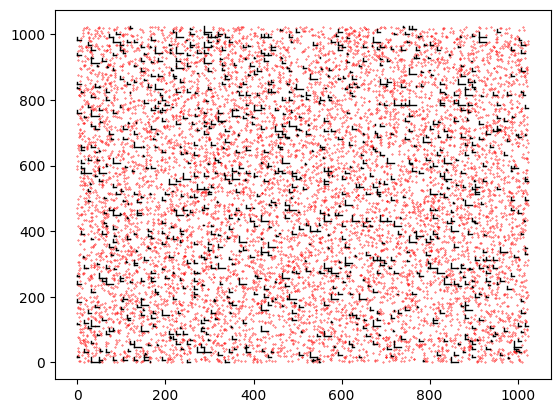
\includegraphics[width=\linewidth]{img/1proc.png}
      \caption{makymalny rząd równy 1}
      \label{fig:obraz1}
  \end{subfigure}
  \hfill
  \begin{subfigure}[b]{0.4\textwidth}
      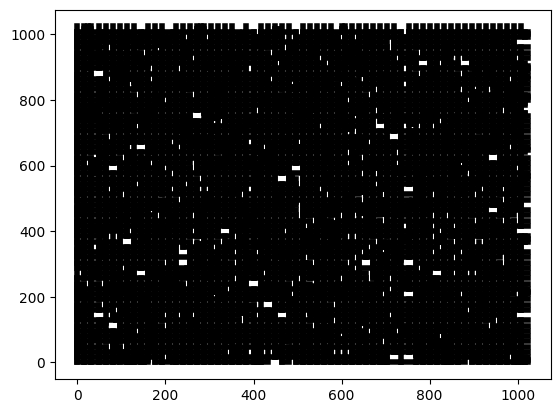
\includegraphics[width=\linewidth]{img/1proc4.png}
      \caption{makymalny rząd równy 4}
      \label{fig:obraz2}
  \end{subfigure}
  \caption{gęstości równa 1 procent}
  \label{fig:zestaw_obrazkow}
\end{figure}
\begin{figure}[htbp]
  \centering
  \begin{subfigure}[b]{0.4\textwidth}
      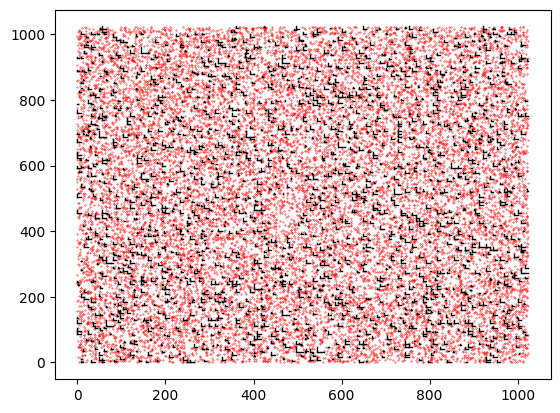
\includegraphics[width=\linewidth]{img/2proc.png}
      \caption{makymalny rząd równy 1}
      \label{fig:obraz1}
  \end{subfigure}
  \hfill
  \begin{subfigure}[b]{0.4\textwidth}
      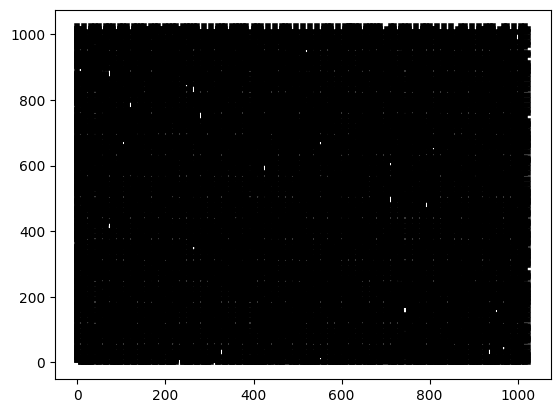
\includegraphics[width=\linewidth]{img/2proc4.png}
      \caption{makymalny rząd równy 4}
      \label{fig:obraz2}
  \end{subfigure}
  \caption{gęstości równa 2 procent}
  \label{fig:zestaw_obrazkow}
\end{figure}

Na rysunkach 1 i 2 można zauważyć, że dla niższego rzędu występują czerwone punkty. Oznaczają one zatrzymanie algorytmu na końcowym warunku dla macierzy o rozmiarze 1x1. Obserwuje się również dużą ilość małych kompresji SVD.
\FloatBarrier
\begin{figure}[htbp]
  \centering
  \begin{subfigure}[b]{0.4\textwidth}
      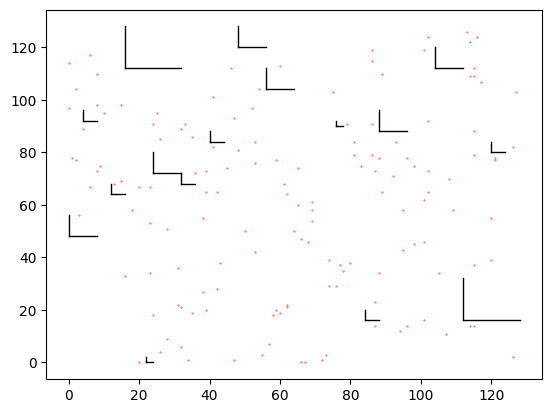
\includegraphics[width=\linewidth]{img/nice_one1.png}
      \caption{makymalny rząd równy 1}
      \label{fig:obraz1}
  \end{subfigure}
  \hfill
  \begin{subfigure}[b]{0.4\textwidth}
      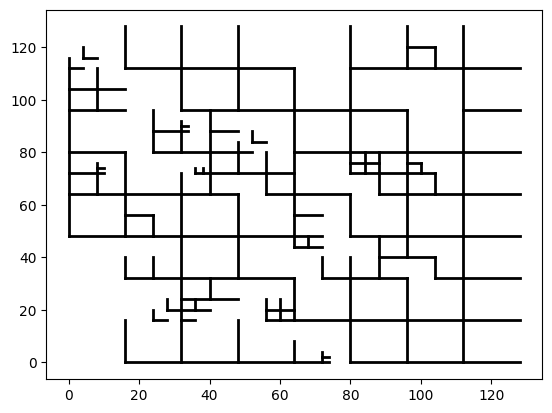
\includegraphics[width=\linewidth]{img/nice_one2.png}
      \caption{makymalny rząd równy 2}
      \label{fig:obraz2}
  \end{subfigure}
  \caption{Dobrze zrobione SVD}
  \label{fig:zestaw_obrazkow}
\end{figure}


Na rysunku 3, w przeciwieństwie do poprzednich, wielkość poszczególnych kompresji jest znaczna względem całej długości boku. Dane wejściowe dla rysunków 1, 2 oraz 3 różnią się wielkością macierzy; w pierwszych dwóch przypadkach jest ona 8 razy większa.

\FloatBarrier
\subsection{Czasy komprescji}

\begin{figure}
  \centering
  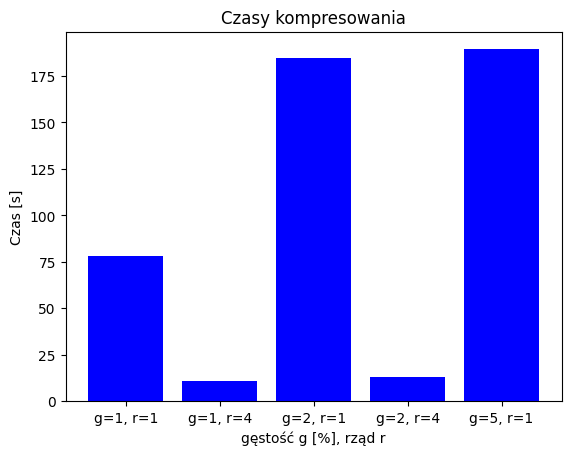
\includegraphics[width=0.9\textwidth]{img/czasy.png}
  \caption{Wykres słupkowy rodzaju kompresji od czasu}
\end{figure}


Jak widać na wykresie 4, zwiększenie dopuszczalnego rzędu macierzy znacznie 
skraca czas kompresji.
 Obserwuje się również tendencję wzrostową w zagęszczaniu macierzy od upływem czasu.

\FloatBarrier
\subsection{Błędy stratności komprescji}
\begin{figure}
  \centering
  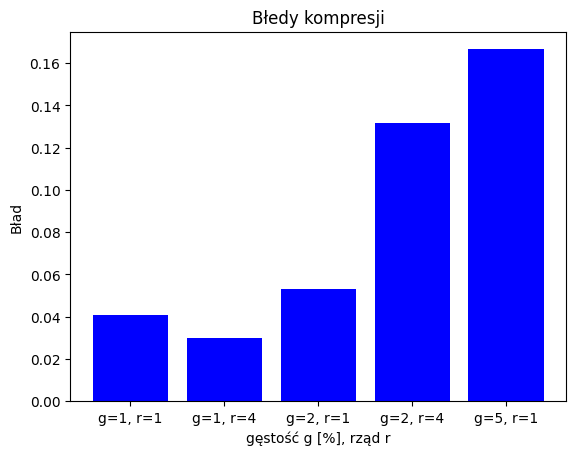
\includegraphics[width=0.9\textwidth]{img/bledy.png}
  \caption{Wykres słupkowy rodzaju kompresji od błędu kwadratowego}
\end{figure}

Widoczne jest, że dla przyjętego epsilonu otrzymywane błędy są znaczące, sięgające
 nawet 0.16. Biorąc pod uwagę, że wartości w macierzach znajdują się w przedziale <0,1>,
  wydaje się, że ta forma kompresji jest kiepskim pomysłem.

Otrzymane wyniki są prawdopodobnie spowodowane zbyt dużą wartością epsilonu, której
 dobór był zbyt wysoki w celu przyspieszenia obliczeń.
\FloatBarrier


\end{document}